\documentclass{standalone}
\usepackage{tikz}
\usetikzlibrary{patterns, positioning}

\begin{document}
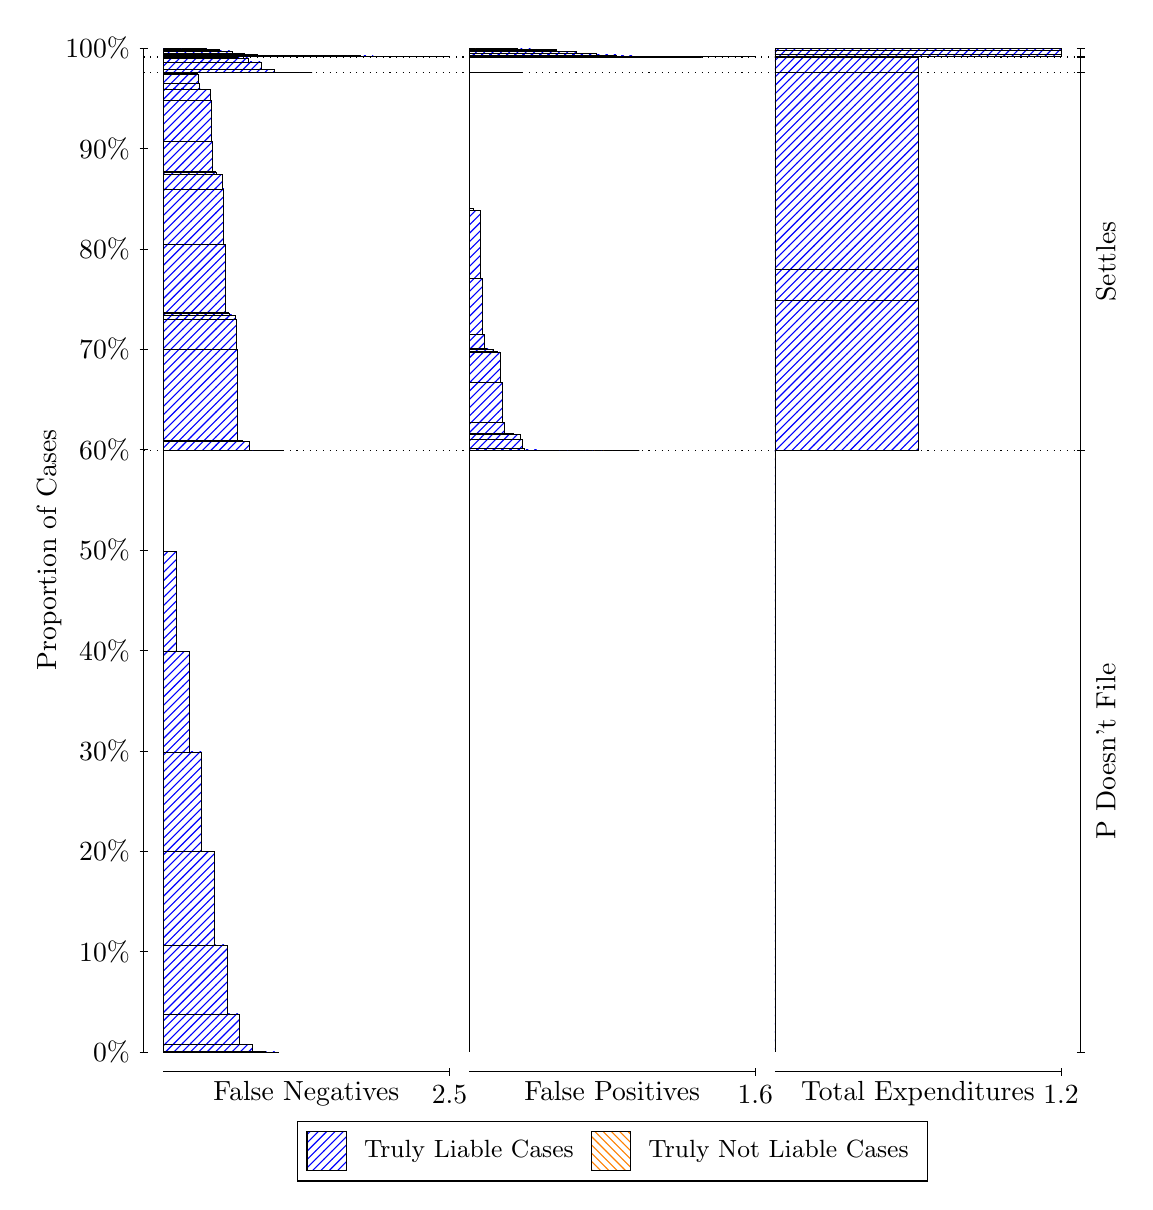
\begin{tikzpicture}
\draw[black, very thin] (1.5,1.75) -- (1.5,14.5);
\node[rotate=90, anchor=center] at (0.3, 8.125) {Proportion of Cases};
\draw[black, very thin] (1.45,1.75) -- (1.55,1.75);
\node[anchor=east] at (1.45, 1.75) {0\%};
\draw[black, very thin] (1.45,3.025) -- (1.55,3.025);
\node[anchor=east] at (1.45, 3.025) {10\%};
\draw[black, very thin] (1.45,4.3) -- (1.55,4.3);
\node[anchor=east] at (1.45, 4.3) {20\%};
\draw[black, very thin] (1.45,5.575) -- (1.55,5.575);
\node[anchor=east] at (1.45, 5.575) {30\%};
\draw[black, very thin] (1.45,6.85) -- (1.55,6.85);
\node[anchor=east] at (1.45, 6.85) {40\%};
\draw[black, very thin] (1.45,8.125) -- (1.55,8.125);
\node[anchor=east] at (1.45, 8.125) {50\%};
\draw[black, very thin] (1.45,9.4) -- (1.55,9.4);
\node[anchor=east] at (1.45, 9.4) {60\%};
\draw[black, very thin] (1.45,10.675) -- (1.55,10.675);
\node[anchor=east] at (1.45, 10.675) {70\%};
\draw[black, very thin] (1.45,11.95) -- (1.55,11.95);
\node[anchor=east] at (1.45, 11.95) {80\%};
\draw[black, very thin] (1.45,13.225) -- (1.55,13.225);
\node[anchor=east] at (1.45, 13.225) {90\%};
\draw[black, very thin] (1.45,14.5) -- (1.55,14.5);
\node[anchor=east] at (1.45, 14.5) {100\%};

\draw[black, very thin] (13.4,1.75) -- (13.4,14.5);
\draw[black, very thin] (13.35,1.75) -- (13.45,1.75);
\node[anchor=west] at (13.35, 1.75) {};
\draw[black, very thin] (13.35,9.3865) -- (13.45,9.3865);
\node[anchor=west] at (13.35, 9.3865) {};
\draw[black, very thin] (13.35,14.19) -- (13.45,14.19);
\node[anchor=west] at (13.35, 14.19) {};
\draw[black, very thin] (13.35,14.384) -- (13.45,14.384);
\node[anchor=west] at (13.35, 14.384) {};
\draw[black, very thin] (13.35,14.397) -- (13.45,14.397);
\node[anchor=west] at (13.35, 14.397) {};
\draw[black, very thin] (13.35,14.5) -- (13.45,14.5);
\node[anchor=west] at (13.35, 14.5) {};

\draw[black, very thin, pattern color=blue, pattern=north east lines] (1.75,1.75) rectangle (3.2033,1.7504);
\draw[black, very thin, pattern color=blue, pattern=north east lines] (1.75,1.7504) rectangle (3.0419,1.7588);
\draw[black, very thin, pattern color=blue, pattern=north east lines] (1.75,1.7588) rectangle (2.8804,1.8436);
\draw[black, very thin, pattern color=blue, pattern=north east lines] (1.75,1.8436) rectangle (2.7189,2.2335);
\draw[black, very thin, pattern color=blue, pattern=north east lines] (1.75,2.2335) rectangle (2.5574,3.1095);
\draw[black, very thin, pattern color=blue, pattern=north east lines] (1.75,3.1095) rectangle (2.3959,4.2957);
\draw[black, very thin, pattern color=blue, pattern=north east lines] (1.75,4.2957) rectangle (2.2344,5.5619);
\draw[black, very thin, pattern color=blue, pattern=north east lines] (1.75,5.5619) rectangle (2.073,6.8365);
\draw[black, very thin, pattern color=blue, pattern=north east lines] (1.75,6.8365) rectangle (1.9115,8.1115);
\draw[black, very thin, pattern color=orange, pattern=north west lines] (1.75,8.1115) rectangle (1.75,8.1115);
\draw[black, very thin, pattern color=blue, pattern=north east lines] (1.75,8.1115) rectangle (1.75,9.3865);
\draw[black, very thin, pattern color=blue, pattern=north east lines] (1.75,9.3865) rectangle (3.276,9.3865);
\draw[black, very thin, pattern color=blue, pattern=north east lines] (1.75,9.3865) rectangle (3.2033,9.3865);
\draw[black, very thin, pattern color=blue, pattern=north east lines] (1.75,9.3865) rectangle (3.1307,9.3865);
\draw[black, very thin, pattern color=blue, pattern=north east lines] (1.75,9.3865) rectangle (3.1145,9.3865);
\draw[black, very thin, pattern color=blue, pattern=north east lines] (1.75,9.3865) rectangle (3.058,9.3865);
\draw[black, very thin, pattern color=blue, pattern=north east lines] (1.75,9.3865) rectangle (3.0419,9.3865);
\draw[black, very thin, pattern color=blue, pattern=north east lines] (1.75,9.3865) rectangle (2.9853,9.3866);
\draw[black, very thin, pattern color=blue, pattern=north east lines] (1.75,9.3866) rectangle (2.9692,9.3866);
\draw[black, very thin, pattern color=blue, pattern=north east lines] (1.75,9.3866) rectangle (2.953,9.3866);
\draw[black, very thin, pattern color=blue, pattern=north east lines] (1.75,9.3866) rectangle (2.9127,9.3874);
\draw[black, very thin, pattern color=blue, pattern=north east lines] (1.75,9.3874) rectangle (2.8965,9.3874);
\draw[black, very thin, pattern color=blue, pattern=north east lines] (1.75,9.3874) rectangle (2.8804,9.3874);
\draw[black, very thin, pattern color=blue, pattern=north east lines] (1.75,9.3874) rectangle (2.84,9.5044);
\draw[black, very thin, pattern color=blue, pattern=north east lines] (1.75,9.5044) rectangle (2.8239,9.507);
\draw[black, very thin, pattern color=blue, pattern=north east lines] (1.75,9.507) rectangle (2.8077,9.5071);
\draw[black, very thin, pattern color=blue, pattern=north east lines] (1.75,9.5071) rectangle (2.7916,9.5072);
\draw[black, very thin, pattern color=blue, pattern=north east lines] (1.75,9.5072) rectangle (2.7512,9.5134);
\draw[black, very thin, pattern color=blue, pattern=north east lines] (1.75,9.5134) rectangle (2.735,9.5149);
\draw[black, very thin, pattern color=blue, pattern=north east lines] (1.75,9.5149) rectangle (2.7189,9.515);
\draw[black, very thin, pattern color=blue, pattern=north east lines] (1.75,9.515) rectangle (2.6947,10.671);
\draw[black, very thin, pattern color=blue, pattern=north east lines] (1.75,10.671) rectangle (2.6785,11.061);
\draw[black, very thin, pattern color=blue, pattern=north east lines] (1.75,11.061) rectangle (2.6624,11.108);
\draw[black, very thin, pattern color=blue, pattern=north east lines] (1.75,11.108) rectangle (2.6462,11.11);
\draw[black, very thin, pattern color=blue, pattern=north east lines] (1.75,11.11) rectangle (2.6301,11.111);
\draw[black, very thin, pattern color=blue, pattern=north east lines] (1.75,11.111) rectangle (2.5897,11.133);
\draw[black, very thin, pattern color=blue, pattern=north east lines] (1.75,11.133) rectangle (2.5736,11.142);
\draw[black, very thin, pattern color=blue, pattern=north east lines] (1.75,11.142) rectangle (2.5574,11.142);
\draw[black, very thin, pattern color=blue, pattern=north east lines] (1.75,11.142) rectangle (2.5332,12.005);
\draw[black, very thin, pattern color=blue, pattern=north east lines] (1.75,12.005) rectangle (2.517,12.71);
\draw[black, very thin, pattern color=blue, pattern=north east lines] (1.75,12.71) rectangle (2.5009,12.893);
\draw[black, very thin, pattern color=blue, pattern=north east lines] (1.75,12.893) rectangle (2.4847,12.898);
\draw[black, very thin, pattern color=blue, pattern=north east lines] (1.75,12.898) rectangle (2.4686,12.899);
\draw[black, very thin, pattern color=blue, pattern=north east lines] (1.75,12.899) rectangle (2.4282,12.925);
\draw[black, very thin, pattern color=blue, pattern=north east lines] (1.75,12.925) rectangle (2.4121,12.933);
\draw[black, very thin, pattern color=blue, pattern=north east lines] (1.75,12.933) rectangle (2.3959,12.934);
\draw[black, very thin, pattern color=blue, pattern=north east lines] (1.75,12.934) rectangle (2.3717,13.316);
\draw[black, very thin, pattern color=blue, pattern=north east lines] (1.75,13.316) rectangle (2.3556,13.832);
\draw[black, very thin, pattern color=blue, pattern=north east lines] (1.75,13.832) rectangle (2.3394,13.971);
\draw[black, very thin, pattern color=blue, pattern=north east lines] (1.75,13.971) rectangle (2.3233,13.973);
\draw[black, very thin, pattern color=blue, pattern=north east lines] (1.75,13.973) rectangle (2.3071,13.974);
\draw[black, very thin, pattern color=blue, pattern=north east lines] (1.75,13.974) rectangle (2.2667,13.981);
\draw[black, very thin, pattern color=blue, pattern=north east lines] (1.75,13.981) rectangle (2.2506,13.982);
\draw[black, very thin, pattern color=blue, pattern=north east lines] (1.75,13.982) rectangle (2.2344,13.982);
\draw[black, very thin, pattern color=blue, pattern=north east lines] (1.75,13.982) rectangle (2.2102,14.05);
\draw[black, very thin, pattern color=blue, pattern=north east lines] (1.75,14.05) rectangle (2.1941,14.161);
\draw[black, very thin, pattern color=blue, pattern=north east lines] (1.75,14.161) rectangle (2.1779,14.18);
\draw[black, very thin, pattern color=blue, pattern=north east lines] (1.75,14.18) rectangle (2.1618,14.181);
\draw[black, very thin, pattern color=blue, pattern=north east lines] (1.75,14.181) rectangle (2.1456,14.181);
\draw[black, very thin, pattern color=blue, pattern=north east lines] (1.75,14.181) rectangle (2.1053,14.181);
\draw[black, very thin, pattern color=blue, pattern=north east lines] (1.75,14.181) rectangle (2.0891,14.181);
\draw[black, very thin, pattern color=blue, pattern=north east lines] (1.75,14.181) rectangle (2.073,14.181);
\draw[black, very thin, pattern color=blue, pattern=north east lines] (1.75,14.181) rectangle (2.0487,14.184);
\draw[black, very thin, pattern color=blue, pattern=north east lines] (1.75,14.184) rectangle (2.0326,14.19);
\draw[black, very thin, pattern color=blue, pattern=north east lines] (1.75,14.19) rectangle (2.0164,14.19);
\draw[black, very thin, pattern color=blue, pattern=north east lines] (1.75,14.19) rectangle (2.0003,14.19);
\draw[black, very thin, pattern color=blue, pattern=north east lines] (1.75,14.19) rectangle (1.9841,14.19);
\draw[black, very thin, pattern color=blue, pattern=north east lines] (1.75,14.19) rectangle (1.9438,14.19);
\draw[black, very thin, pattern color=blue, pattern=north east lines] (1.75,14.19) rectangle (1.9276,14.19);
\draw[black, very thin, pattern color=blue, pattern=north east lines] (1.75,14.19) rectangle (1.9115,14.19);
\draw[black, very thin, pattern color=blue, pattern=north east lines] (1.75,14.19) rectangle (1.8873,14.19);
\draw[black, very thin, pattern color=blue, pattern=north east lines] (1.75,14.19) rectangle (1.8711,14.19);
\draw[black, very thin, pattern color=blue, pattern=north east lines] (1.75,14.19) rectangle (1.855,14.19);
\draw[black, very thin, pattern color=blue, pattern=north east lines] (1.75,14.19) rectangle (1.8388,14.19);
\draw[black, very thin, pattern color=blue, pattern=north east lines] (1.75,14.19) rectangle (1.8227,14.19);
\draw[black, very thin, pattern color=blue, pattern=north east lines] (1.75,14.19) rectangle (1.7823,14.19);
\draw[black, very thin, pattern color=blue, pattern=north east lines] (1.75,14.19) rectangle (1.7661,14.19);
\draw[black, very thin, pattern color=orange, pattern=north west lines] (1.75,14.19) rectangle (1.75,14.19);
\draw[black, very thin, pattern color=blue, pattern=north east lines] (1.75,14.19) rectangle (1.75,14.19);
\draw[black, very thin, pattern color=blue, pattern=north east lines] (1.75,14.19) rectangle (3.6393,14.19);
\draw[black, very thin, pattern color=blue, pattern=north east lines] (1.75,14.19) rectangle (3.4779,14.19);
\draw[black, very thin, pattern color=blue, pattern=north east lines] (1.75,14.19) rectangle (3.3164,14.194);
\draw[black, very thin, pattern color=blue, pattern=north east lines] (1.75,14.194) rectangle (3.1549,14.229);
\draw[black, very thin, pattern color=blue, pattern=north east lines] (1.75,14.229) rectangle (2.9934,14.323);
\draw[black, very thin, pattern color=blue, pattern=north east lines] (1.75,14.323) rectangle (2.8319,14.376);
\draw[black, very thin, pattern color=blue, pattern=north east lines] (1.75,14.376) rectangle (2.6704,14.384);
\draw[black, very thin, pattern color=blue, pattern=north east lines] (1.75,14.384) rectangle (2.509,14.384);
\draw[black, very thin, pattern color=blue, pattern=north east lines] (1.75,14.384) rectangle (2.3475,14.384);
\draw[black, very thin, pattern color=blue, pattern=north east lines] (1.75,14.384) rectangle (2.186,14.384);
\draw[black, very thin, pattern color=orange, pattern=north west lines] (1.75,14.384) rectangle (1.75,14.384);
\draw[black, very thin, pattern color=blue, pattern=north east lines] (1.75,14.384) rectangle (2.186,14.385);
\draw[black, very thin, pattern color=blue, pattern=north east lines] (1.75,14.385) rectangle (2.0245,14.386);
\draw[black, very thin, pattern color=blue, pattern=north east lines] (1.75,14.386) rectangle (1.863,14.391);
\draw[black, very thin, pattern color=orange, pattern=north west lines] (1.75,14.391) rectangle (1.75,14.391);
\draw[black, very thin, pattern color=blue, pattern=north east lines] (1.75,14.391) rectangle (1.75,14.397);
\draw[black, very thin, pattern color=blue, pattern=north east lines] (1.75,14.397) rectangle (5.3833,14.397);
\draw[black, very thin, pattern color=blue, pattern=north east lines] (1.75,14.397) rectangle (5.2219,14.397);
\draw[black, very thin, pattern color=blue, pattern=north east lines] (1.75,14.397) rectangle (5.0604,14.397);
\draw[black, very thin, pattern color=blue, pattern=north east lines] (1.75,14.397) rectangle (4.8989,14.397);
\draw[black, very thin, pattern color=blue, pattern=north east lines] (1.75,14.397) rectangle (4.8989,14.397);
\draw[black, very thin, pattern color=blue, pattern=north east lines] (1.75,14.397) rectangle (4.7374,14.398);
\draw[black, very thin, pattern color=blue, pattern=north east lines] (1.75,14.398) rectangle (4.5759,14.398);
\draw[black, very thin, pattern color=blue, pattern=north east lines] (1.75,14.398) rectangle (4.5759,14.398);
\draw[black, very thin, pattern color=blue, pattern=north east lines] (1.75,14.398) rectangle (4.5759,14.398);
\draw[black, very thin, pattern color=blue, pattern=north east lines] (1.75,14.398) rectangle (4.4144,14.4);
\draw[black, very thin, pattern color=blue, pattern=north east lines] (1.75,14.4) rectangle (4.4144,14.401);
\draw[black, very thin, pattern color=blue, pattern=north east lines] (1.75,14.401) rectangle (4.253,14.405);
\draw[black, very thin, pattern color=blue, pattern=north east lines] (1.75,14.405) rectangle (4.253,14.405);
\draw[black, very thin, pattern color=blue, pattern=north east lines] (1.75,14.405) rectangle (4.0915,14.406);
\draw[black, very thin, pattern color=blue, pattern=north east lines] (1.75,14.406) rectangle (4.0915,14.406);
\draw[black, very thin, pattern color=blue, pattern=north east lines] (1.75,14.406) rectangle (3.93,14.406);
\draw[black, very thin, pattern color=blue, pattern=north east lines] (1.75,14.406) rectangle (3.7685,14.406);
\draw[black, very thin, pattern color=blue, pattern=north east lines] (1.75,14.406) rectangle (3.7524,14.406);
\draw[black, very thin, pattern color=blue, pattern=north east lines] (1.75,14.406) rectangle (3.607,14.406);
\draw[black, very thin, pattern color=blue, pattern=north east lines] (1.75,14.406) rectangle (3.607,14.406);
\draw[black, very thin, pattern color=blue, pattern=north east lines] (1.75,14.406) rectangle (3.5909,14.406);
\draw[black, very thin, pattern color=blue, pattern=north east lines] (1.75,14.406) rectangle (3.4456,14.406);
\draw[black, very thin, pattern color=blue, pattern=north east lines] (1.75,14.406) rectangle (3.4294,14.406);
\draw[black, very thin, pattern color=blue, pattern=north east lines] (1.75,14.406) rectangle (3.2841,14.406);
\draw[black, very thin, pattern color=blue, pattern=north east lines] (1.75,14.406) rectangle (3.2679,14.406);
\draw[black, very thin, pattern color=blue, pattern=north east lines] (1.75,14.406) rectangle (3.2679,14.406);
\draw[black, very thin, pattern color=blue, pattern=north east lines] (1.75,14.406) rectangle (3.1064,14.407);
\draw[black, very thin, pattern color=blue, pattern=north east lines] (1.75,14.407) rectangle (3.1064,14.407);
\draw[black, very thin, pattern color=blue, pattern=north east lines] (1.75,14.407) rectangle (2.945,14.415);
\draw[black, very thin, pattern color=blue, pattern=north east lines] (1.75,14.415) rectangle (2.7835,14.426);
\draw[black, very thin, pattern color=blue, pattern=north east lines] (1.75,14.426) rectangle (2.7835,14.436);
\draw[black, very thin, pattern color=blue, pattern=north east lines] (1.75,14.436) rectangle (2.622,14.464);
\draw[black, very thin, pattern color=blue, pattern=north east lines] (1.75,14.464) rectangle (2.4605,14.475);
\draw[black, very thin, pattern color=blue, pattern=north east lines] (1.75,14.475) rectangle (2.4605,14.475);
\draw[black, very thin, pattern color=blue, pattern=north east lines] (1.75,14.475) rectangle (2.4605,14.486);
\draw[black, very thin, pattern color=blue, pattern=north east lines] (1.75,14.486) rectangle (2.299,14.497);
\draw[black, very thin, pattern color=blue, pattern=north east lines] (1.75,14.497) rectangle (2.299,14.497);
\draw[black, very thin, pattern color=blue, pattern=north east lines] (1.75,14.497) rectangle (2.1376,14.498);
\draw[black, very thin, pattern color=blue, pattern=north east lines] (1.75,14.498) rectangle (2.1376,14.498);
\draw[black, very thin, pattern color=blue, pattern=north east lines] (1.75,14.498) rectangle (2.1376,14.5);
\draw[black, very thin, pattern color=blue, pattern=north east lines] (1.75,14.5) rectangle (1.9761,14.5);
\draw[black, very thin, pattern color=blue, pattern=north east lines] (1.75,14.5) rectangle (1.9761,14.5);
\draw[black, very thin, pattern color=blue, pattern=north east lines] (1.75,14.5) rectangle (1.8146,14.5);
\draw[black, very thin, pattern color=blue, pattern=north east lines] (1.75,14.5) rectangle (1.8146,14.5);
\draw[black, very thin, pattern color=orange, pattern=north west lines] (1.75,14.5) rectangle (1.75,14.5);
\draw[black, very thin, pattern color=blue, pattern=north east lines] (1.75,14.5) rectangle (1.75,14.5);
\draw[black, very thin, pattern color=orange, pattern=north west lines] (5.6333,1.75) rectangle (5.6333,1.75);
\draw[black, very thin, pattern color=blue, pattern=north east lines] (5.6333,1.75) rectangle (5.6333,9.3865);
\draw[black, very thin, pattern color=orange, pattern=north west lines] (5.6333,9.3865) rectangle (7.7906,9.3865);
\draw[black, very thin, pattern color=blue, pattern=north east lines] (5.6333,9.3865) rectangle (7.7906,9.3865);
\draw[black, very thin, pattern color=orange, pattern=north west lines] (5.6333,9.3865) rectangle (7.5635,9.3865);
\draw[black, very thin, pattern color=blue, pattern=north east lines] (5.6333,9.3865) rectangle (7.5635,9.3865);
\draw[black, very thin, pattern color=blue, pattern=north east lines] (5.6333,9.3865) rectangle (7.5383,9.3865);
\draw[black, very thin, pattern color=orange, pattern=north west lines] (5.6333,9.3865) rectangle (7.45,9.3865);
\draw[black, very thin, pattern color=blue, pattern=north east lines] (5.6333,9.3865) rectangle (7.45,9.3865);
\draw[black, very thin, pattern color=orange, pattern=north west lines] (5.6333,9.3865) rectangle (7.3365,9.3865);
\draw[black, very thin, pattern color=blue, pattern=north east lines] (5.6333,9.3865) rectangle (7.3365,9.3865);
\draw[black, very thin, pattern color=blue, pattern=north east lines] (5.6333,9.3865) rectangle (7.3112,9.3865);
\draw[black, very thin, pattern color=blue, pattern=north east lines] (5.6333,9.3865) rectangle (7.286,9.3865);
\draw[black, very thin, pattern color=orange, pattern=north west lines] (5.6333,9.3865) rectangle (7.2229,9.3865);
\draw[black, very thin, pattern color=blue, pattern=north east lines] (5.6333,9.3865) rectangle (7.2229,9.3865);
\draw[black, very thin, pattern color=blue, pattern=north east lines] (5.6333,9.3865) rectangle (7.1977,9.3865);
\draw[black, very thin, pattern color=orange, pattern=north west lines] (5.6333,9.3865) rectangle (7.1094,9.3865);
\draw[black, very thin, pattern color=blue, pattern=north east lines] (5.6333,9.3865) rectangle (7.1094,9.3865);
\draw[black, very thin, pattern color=blue, pattern=north east lines] (5.6333,9.3865) rectangle (7.0841,9.3865);
\draw[black, very thin, pattern color=blue, pattern=north east lines] (5.6333,9.3865) rectangle (7.0589,9.3865);
\draw[black, very thin, pattern color=blue, pattern=north east lines] (5.6333,9.3865) rectangle (7.0337,9.3865);
\draw[black, very thin, pattern color=orange, pattern=north west lines] (5.6333,9.3865) rectangle (6.9958,9.3865);
\draw[black, very thin, pattern color=blue, pattern=north east lines] (5.6333,9.3865) rectangle (6.9958,9.3865);
\draw[black, very thin, pattern color=blue, pattern=north east lines] (5.6333,9.3865) rectangle (6.9706,9.3865);
\draw[black, very thin, pattern color=blue, pattern=north east lines] (5.6333,9.3865) rectangle (6.9454,9.3865);
\draw[black, very thin, pattern color=orange, pattern=north west lines] (5.6333,9.3865) rectangle (6.8823,9.3865);
\draw[black, very thin, pattern color=blue, pattern=north east lines] (5.6333,9.3865) rectangle (6.8823,9.3865);
\draw[black, very thin, pattern color=blue, pattern=north east lines] (5.6333,9.3865) rectangle (6.8571,9.3865);
\draw[black, very thin, pattern color=blue, pattern=north east lines] (5.6333,9.3865) rectangle (6.8318,9.3865);
\draw[black, very thin, pattern color=blue, pattern=north east lines] (5.6333,9.3865) rectangle (6.8066,9.3866);
\draw[black, very thin, pattern color=blue, pattern=north east lines] (5.6333,9.3866) rectangle (6.7814,9.3866);
\draw[black, very thin, pattern color=blue, pattern=north east lines] (5.6333,9.3866) rectangle (6.7435,9.3866);
\draw[black, very thin, pattern color=blue, pattern=north east lines] (5.6333,9.3866) rectangle (6.7183,9.3866);
\draw[black, very thin, pattern color=blue, pattern=north east lines] (5.6333,9.3866) rectangle (6.6931,9.3866);
\draw[black, very thin, pattern color=blue, pattern=north east lines] (5.6333,9.3866) rectangle (6.63,9.3866);
\draw[black, very thin, pattern color=blue, pattern=north east lines] (5.6333,9.3866) rectangle (6.6047,9.3866);
\draw[black, very thin, pattern color=blue, pattern=north east lines] (5.6333,9.3866) rectangle (6.5795,9.3871);
\draw[black, very thin, pattern color=blue, pattern=north east lines] (5.6333,9.3871) rectangle (6.5543,9.3923);
\draw[black, very thin, pattern color=blue, pattern=north east lines] (5.6333,9.3923) rectangle (6.5291,9.3958);
\draw[black, very thin, pattern color=blue, pattern=north east lines] (5.6333,9.3958) rectangle (6.4912,9.3958);
\draw[black, very thin, pattern color=blue, pattern=north east lines] (5.6333,9.3958) rectangle (6.466,9.3958);
\draw[black, very thin, pattern color=blue, pattern=north east lines] (5.6333,9.3958) rectangle (6.4407,9.3962);
\draw[black, very thin, pattern color=blue, pattern=north east lines] (5.6333,9.3962) rectangle (6.3777,9.3962);
\draw[black, very thin, pattern color=blue, pattern=north east lines] (5.6333,9.3962) rectangle (6.3524,9.3964);
\draw[black, very thin, pattern color=blue, pattern=north east lines] (5.6333,9.3964) rectangle (6.3272,9.4156);
\draw[black, very thin, pattern color=blue, pattern=north east lines] (5.6333,9.4156) rectangle (6.302,9.5263);
\draw[black, very thin, pattern color=blue, pattern=north east lines] (5.6333,9.5263) rectangle (6.2767,9.5945);
\draw[black, very thin, pattern color=blue, pattern=north east lines] (5.6333,9.5945) rectangle (6.2389,9.5946);
\draw[black, very thin, pattern color=blue, pattern=north east lines] (5.6333,9.5946) rectangle (6.2137,9.596);
\draw[black, very thin, pattern color=blue, pattern=north east lines] (5.6333,9.596) rectangle (6.1884,9.6032);
\draw[black, very thin, pattern color=blue, pattern=north east lines] (5.6333,9.6032) rectangle (6.1253,9.6034);
\draw[black, very thin, pattern color=blue, pattern=north east lines] (5.6333,9.6034) rectangle (6.1001,9.6055);
\draw[black, very thin, pattern color=blue, pattern=north east lines] (5.6333,9.6055) rectangle (6.0749,9.7446);
\draw[black, very thin, pattern color=blue, pattern=north east lines] (5.6333,9.7446) rectangle (6.0497,10.26);
\draw[black, very thin, pattern color=blue, pattern=north east lines] (5.6333,10.26) rectangle (6.0244,10.642);
\draw[black, very thin, pattern color=blue, pattern=north east lines] (5.6333,10.642) rectangle (5.9866,10.643);
\draw[black, very thin, pattern color=blue, pattern=north east lines] (5.6333,10.643) rectangle (5.9613,10.652);
\draw[black, very thin, pattern color=blue, pattern=north east lines] (5.6333,10.652) rectangle (5.9361,10.678);
\draw[black, very thin, pattern color=blue, pattern=north east lines] (5.6333,10.678) rectangle (5.873,10.679);
\draw[black, very thin, pattern color=blue, pattern=north east lines] (5.6333,10.679) rectangle (5.8478,10.684);
\draw[black, very thin, pattern color=blue, pattern=north east lines] (5.6333,10.684) rectangle (5.8226,10.867);
\draw[black, very thin, pattern color=blue, pattern=north east lines] (5.6333,10.867) rectangle (5.7973,11.572);
\draw[black, very thin, pattern color=blue, pattern=north east lines] (5.6333,11.572) rectangle (5.7721,12.434);
\draw[black, very thin, pattern color=blue, pattern=north east lines] (5.6333,12.434) rectangle (5.7343,12.435);
\draw[black, very thin, pattern color=blue, pattern=north east lines] (5.6333,12.435) rectangle (5.709,12.444);
\draw[black, very thin, pattern color=blue, pattern=north east lines] (5.6333,12.444) rectangle (5.6838,12.466);
\draw[black, very thin, pattern color=blue, pattern=north east lines] (5.6333,12.466) rectangle (5.6333,14.19);
\draw[black, very thin, pattern color=orange, pattern=north west lines] (5.6333,14.19) rectangle (6.3146,14.19);
\draw[black, very thin, pattern color=blue, pattern=north east lines] (5.6333,14.19) rectangle (6.3146,14.19);
\draw[black, very thin, pattern color=blue, pattern=north east lines] (5.6333,14.19) rectangle (6.0623,14.19);
\draw[black, very thin, pattern color=blue, pattern=north east lines] (5.6333,14.19) rectangle (5.81,14.191);
\draw[black, very thin, pattern color=blue, pattern=north east lines] (5.6333,14.191) rectangle (5.6333,14.384);
\draw[black, very thin, pattern color=orange, pattern=north west lines] (5.6333,14.384) rectangle (8.5854,14.384);
\draw[black, very thin, pattern color=blue, pattern=north east lines] (5.6333,14.384) rectangle (8.5854,14.384);
\draw[black, very thin, pattern color=blue, pattern=north east lines] (5.6333,14.384) rectangle (8.3331,14.384);
\draw[black, very thin, pattern color=blue, pattern=north east lines] (5.6333,14.384) rectangle (8.0808,14.384);
\draw[black, very thin, pattern color=blue, pattern=north east lines] (5.6333,14.384) rectangle (7.8285,14.384);
\draw[black, very thin, pattern color=blue, pattern=north east lines] (5.6333,14.384) rectangle (7.5762,14.384);
\draw[black, very thin, pattern color=blue, pattern=north east lines] (5.6333,14.384) rectangle (7.3238,14.385);
\draw[black, very thin, pattern color=blue, pattern=north east lines] (5.6333,14.385) rectangle (7.0715,14.39);
\draw[black, very thin, pattern color=blue, pattern=north east lines] (5.6333,14.39) rectangle (6.8192,14.396);
\draw[black, very thin, pattern color=blue, pattern=north east lines] (5.6333,14.396) rectangle (6.5669,14.397);
\draw[black, very thin, pattern color=blue, pattern=north east lines] (5.6333,14.397) rectangle (6.3146,14.397);
\draw[black, very thin, pattern color=orange, pattern=north west lines] (5.6333,14.397) rectangle (9.2667,14.397);
\draw[black, very thin, pattern color=blue, pattern=north east lines] (5.6333,14.397) rectangle (9.2667,14.397);
\draw[black, very thin, pattern color=orange, pattern=north west lines] (5.6333,14.397) rectangle (9.0144,14.397);
\draw[black, very thin, pattern color=blue, pattern=north east lines] (5.6333,14.397) rectangle (9.0144,14.397);
\draw[black, very thin, pattern color=orange, pattern=north west lines] (5.6333,14.397) rectangle (8.762,14.397);
\draw[black, very thin, pattern color=blue, pattern=north east lines] (5.6333,14.397) rectangle (8.762,14.397);
\draw[black, very thin, pattern color=blue, pattern=north east lines] (5.6333,14.397) rectangle (8.5097,14.397);
\draw[black, very thin, pattern color=orange, pattern=north west lines] (5.6333,14.397) rectangle (8.5097,14.397);
\draw[black, very thin, pattern color=blue, pattern=north east lines] (5.6333,14.397) rectangle (8.5097,14.397);
\draw[black, very thin, pattern color=blue, pattern=north east lines] (5.6333,14.397) rectangle (8.2574,14.397);
\draw[black, very thin, pattern color=orange, pattern=north west lines] (5.6333,14.397) rectangle (8.2574,14.397);
\draw[black, very thin, pattern color=blue, pattern=north east lines] (5.6333,14.397) rectangle (8.2574,14.397);
\draw[black, very thin, pattern color=blue, pattern=north east lines] (5.6333,14.397) rectangle (8.0051,14.398);
\draw[black, very thin, pattern color=orange, pattern=north west lines] (5.6333,14.398) rectangle (8.0051,14.398);
\draw[black, very thin, pattern color=blue, pattern=north east lines] (5.6333,14.398) rectangle (8.0051,14.398);
\draw[black, very thin, pattern color=blue, pattern=north east lines] (5.6333,14.398) rectangle (7.7528,14.399);
\draw[black, very thin, pattern color=orange, pattern=north west lines] (5.6333,14.399) rectangle (7.7528,14.399);
\draw[black, very thin, pattern color=blue, pattern=north east lines] (5.6333,14.399) rectangle (7.7528,14.401);
\draw[black, very thin, pattern color=blue, pattern=north east lines] (5.6333,14.401) rectangle (7.7528,14.401);
\draw[black, very thin, pattern color=blue, pattern=north east lines] (5.6333,14.401) rectangle (7.7528,14.401);
\draw[black, very thin, pattern color=blue, pattern=north east lines] (5.6333,14.401) rectangle (7.5005,14.408);
\draw[black, very thin, pattern color=orange, pattern=north west lines] (5.6333,14.408) rectangle (7.5005,14.408);
\draw[black, very thin, pattern color=blue, pattern=north east lines] (5.6333,14.408) rectangle (7.5005,14.412);
\draw[black, very thin, pattern color=blue, pattern=north east lines] (5.6333,14.412) rectangle (7.5005,14.412);
\draw[black, very thin, pattern color=blue, pattern=north east lines] (5.6333,14.412) rectangle (7.2481,14.413);
\draw[black, very thin, pattern color=blue, pattern=north east lines] (5.6333,14.413) rectangle (7.2481,14.427);
\draw[black, very thin, pattern color=blue, pattern=north east lines] (5.6333,14.427) rectangle (7.2481,14.434);
\draw[black, very thin, pattern color=blue, pattern=north east lines] (5.6333,14.434) rectangle (6.9958,14.435);
\draw[black, very thin, pattern color=blue, pattern=north east lines] (5.6333,14.435) rectangle (6.9958,14.453);
\draw[black, very thin, pattern color=blue, pattern=north east lines] (5.6333,14.453) rectangle (6.9958,14.461);
\draw[black, very thin, pattern color=blue, pattern=north east lines] (5.6333,14.461) rectangle (6.7435,14.463);
\draw[black, very thin, pattern color=blue, pattern=north east lines] (5.6333,14.463) rectangle (6.7435,14.463);
\draw[black, very thin, pattern color=blue, pattern=north east lines] (5.6333,14.463) rectangle (6.7435,14.477);
\draw[black, very thin, pattern color=blue, pattern=north east lines] (5.6333,14.477) rectangle (6.7435,14.482);
\draw[black, very thin, pattern color=blue, pattern=north east lines] (5.6333,14.482) rectangle (6.4912,14.485);
\draw[black, very thin, pattern color=blue, pattern=north east lines] (5.6333,14.485) rectangle (6.4912,14.49);
\draw[black, very thin, pattern color=blue, pattern=north east lines] (5.6333,14.49) rectangle (6.2389,14.491);
\draw[black, very thin, pattern color=blue, pattern=north east lines] (5.6333,14.491) rectangle (6.2389,14.491);
\draw[black, very thin, pattern color=blue, pattern=north east lines] (5.6333,14.491) rectangle (6.2389,14.491);
\draw[black, very thin, pattern color=blue, pattern=north east lines] (5.6333,14.491) rectangle (5.9866,14.491);
\draw[black, very thin, pattern color=blue, pattern=north east lines] (5.6333,14.491) rectangle (5.9866,14.492);
\draw[black, very thin, pattern color=orange, pattern=north west lines] (5.6333,14.492) rectangle (5.9613,14.492);
\draw[black, very thin, pattern color=blue, pattern=north east lines] (5.6333,14.492) rectangle (5.9613,14.492);
\draw[black, very thin, pattern color=blue, pattern=north east lines] (5.6333,14.492) rectangle (5.7343,14.492);
\draw[black, very thin, pattern color=blue, pattern=north east lines] (5.6333,14.492) rectangle (5.7343,14.492);
\draw[black, very thin, pattern color=blue, pattern=north east lines] (5.6333,14.492) rectangle (5.7343,14.492);
\draw[black, very thin, pattern color=orange, pattern=north west lines] (5.6333,14.492) rectangle (5.709,14.492);
\draw[black, very thin, pattern color=blue, pattern=north east lines] (5.6333,14.492) rectangle (5.709,14.492);
\draw[black, very thin, pattern color=orange, pattern=north west lines] (5.6333,14.492) rectangle (5.6333,14.492);
\draw[black, very thin, pattern color=blue, pattern=north east lines] (5.6333,14.492) rectangle (5.6333,14.5);
\draw[black, very thin, pattern color=orange, pattern=north west lines] (9.5167,1.75) rectangle (9.5167,1.75);
\draw[black, very thin, pattern color=blue, pattern=north east lines] (9.5167,1.75) rectangle (9.5167,9.3865);
\draw[black, very thin, pattern color=orange, pattern=north west lines] (9.5167,9.3865) rectangle (11.333,9.3865);
\draw[black, very thin, pattern color=blue, pattern=north east lines] (9.5167,9.3865) rectangle (11.333,11.294);
\draw[black, very thin, pattern color=orange, pattern=north west lines] (9.5167,11.294) rectangle (11.333,11.294);
\draw[black, very thin, pattern color=blue, pattern=north east lines] (9.5167,11.294) rectangle (11.333,11.687);
\draw[black, very thin, pattern color=orange, pattern=north west lines] (9.5167,11.687) rectangle (11.333,11.687);
\draw[black, very thin, pattern color=blue, pattern=north east lines] (9.5167,11.687) rectangle (11.333,14.19);
\draw[black, very thin, pattern color=orange, pattern=north west lines] (9.5167,14.19) rectangle (11.333,14.19);
\draw[black, very thin, pattern color=blue, pattern=north east lines] (9.5167,14.19) rectangle (11.333,14.384);
\draw[black, very thin, pattern color=orange, pattern=north west lines] (9.5167,14.384) rectangle (11.333,14.384);
\draw[black, very thin, pattern color=blue, pattern=north east lines] (9.5167,14.384) rectangle (11.333,14.397);
\draw[black, very thin, pattern color=orange, pattern=north west lines] (9.5167,14.397) rectangle (13.15,14.397);
\draw[black, very thin, pattern color=blue, pattern=north east lines] (9.5167,14.397) rectangle (13.15,14.422);
\draw[black, very thin, pattern color=orange, pattern=north west lines] (9.5167,14.422) rectangle (13.15,14.422);
\draw[black, very thin, pattern color=blue, pattern=north east lines] (9.5167,14.422) rectangle (13.15,14.47);
\draw[black, very thin, pattern color=orange, pattern=north west lines] (9.5167,14.47) rectangle (13.15,14.47);
\draw[black, very thin, pattern color=blue, pattern=north east lines] (9.5167,14.47) rectangle (13.15,14.5);
\draw[black, dotted] (1.5,9.3865) -- (13.4,9.3865);
\draw[black, dotted] (1.5,14.19) -- (13.4,14.19);
\draw[black, dotted] (1.5,14.384) -- (13.4,14.384);
\draw[black, dotted] (1.5,14.397) -- (13.4,14.397);
\draw[black, very thin] (1.75,1.5) -- (5.3833,1.5);
\node[anchor=north] at (3.5667, 1.5) {False Negatives};
\draw[black, very thin] (5.3833,1.45) -- (5.3833,1.55);
\node[anchor=north] at (5.3833, 1.45) {2.5};

\draw[black, very thin] (5.6333,1.5) -- (9.2667,1.5);
\node[anchor=north] at (7.45, 1.5) {False Positives};
\draw[black, very thin] (9.2667,1.45) -- (9.2667,1.55);
\node[anchor=north] at (9.2667, 1.45) {1.6};

\draw[black, very thin] (9.5167,1.5) -- (13.15,1.5);
\node[anchor=north] at (11.333, 1.5) {Total Expenditures};
\draw[black, very thin] (13.15,1.45) -- (13.15,1.55);
\node[anchor=north] at (13.15, 1.45) {1.2};

\node[black, centered, rotate=90] at (13.72, 5.5683) {P Doesn't File};
\node[black, centered, rotate=90] at (13.72, 11.788) {Settles};




\draw (7.449999999999999,1.5) node[draw=none] (baseCoordinate) {};
\begin{scope}[align=center]
        \matrix[scale=0.5, draw=black, below=0.5cm of baseCoordinate, nodes={draw}, column sep=0.1cm]{
            \node[rectangle, draw, minimum width=0.5cm, minimum height=0.5cm, pattern=north east lines, pattern color=blue] {}; &
            \node[draw=none, font=\small] (B) {Truly Liable Cases}; &
            \node[rectangle, draw, minimum width=0.5cm, minimum height=0.5cm, pattern=north west lines, pattern color=orange] {}; &
            \node[draw=none, font=\small] (B) {Truly Not Liable Cases}; \\
            };
\end{scope}

\end{tikzpicture}
\end{document}